The ANN outputs and discriminant (defined in Eq.~\ref{eq:NN_discriminant}) for the \zdom{} SR are seen in Figures~\ref{fig:vh_wh_zdom_outputs} and~\ref{fig:vh_wh_zdom_discriminant}, respectively, and for the \zdep{} SR in Figures~\ref{fig:vh_wh_zdep_outputs} and~\ref{fig:vh_wh_zdep_discriminant}, respectively. The output nodes of the ANN indicate that the network is performing well since it is successfully identifying its corresponding background by populating the low and high valued bins with the correct MC samples. Additionally, the ANN discriminant is performing well as can be seen in the $WH$ and background separtion in the most sensitive bin.. The binning of the neural network discriminant is subject to optimization in the statistical analysis.

\begin{figure}[htp]
  \centering
  \subfloat[\zdom{} $WH$ output node score]{
    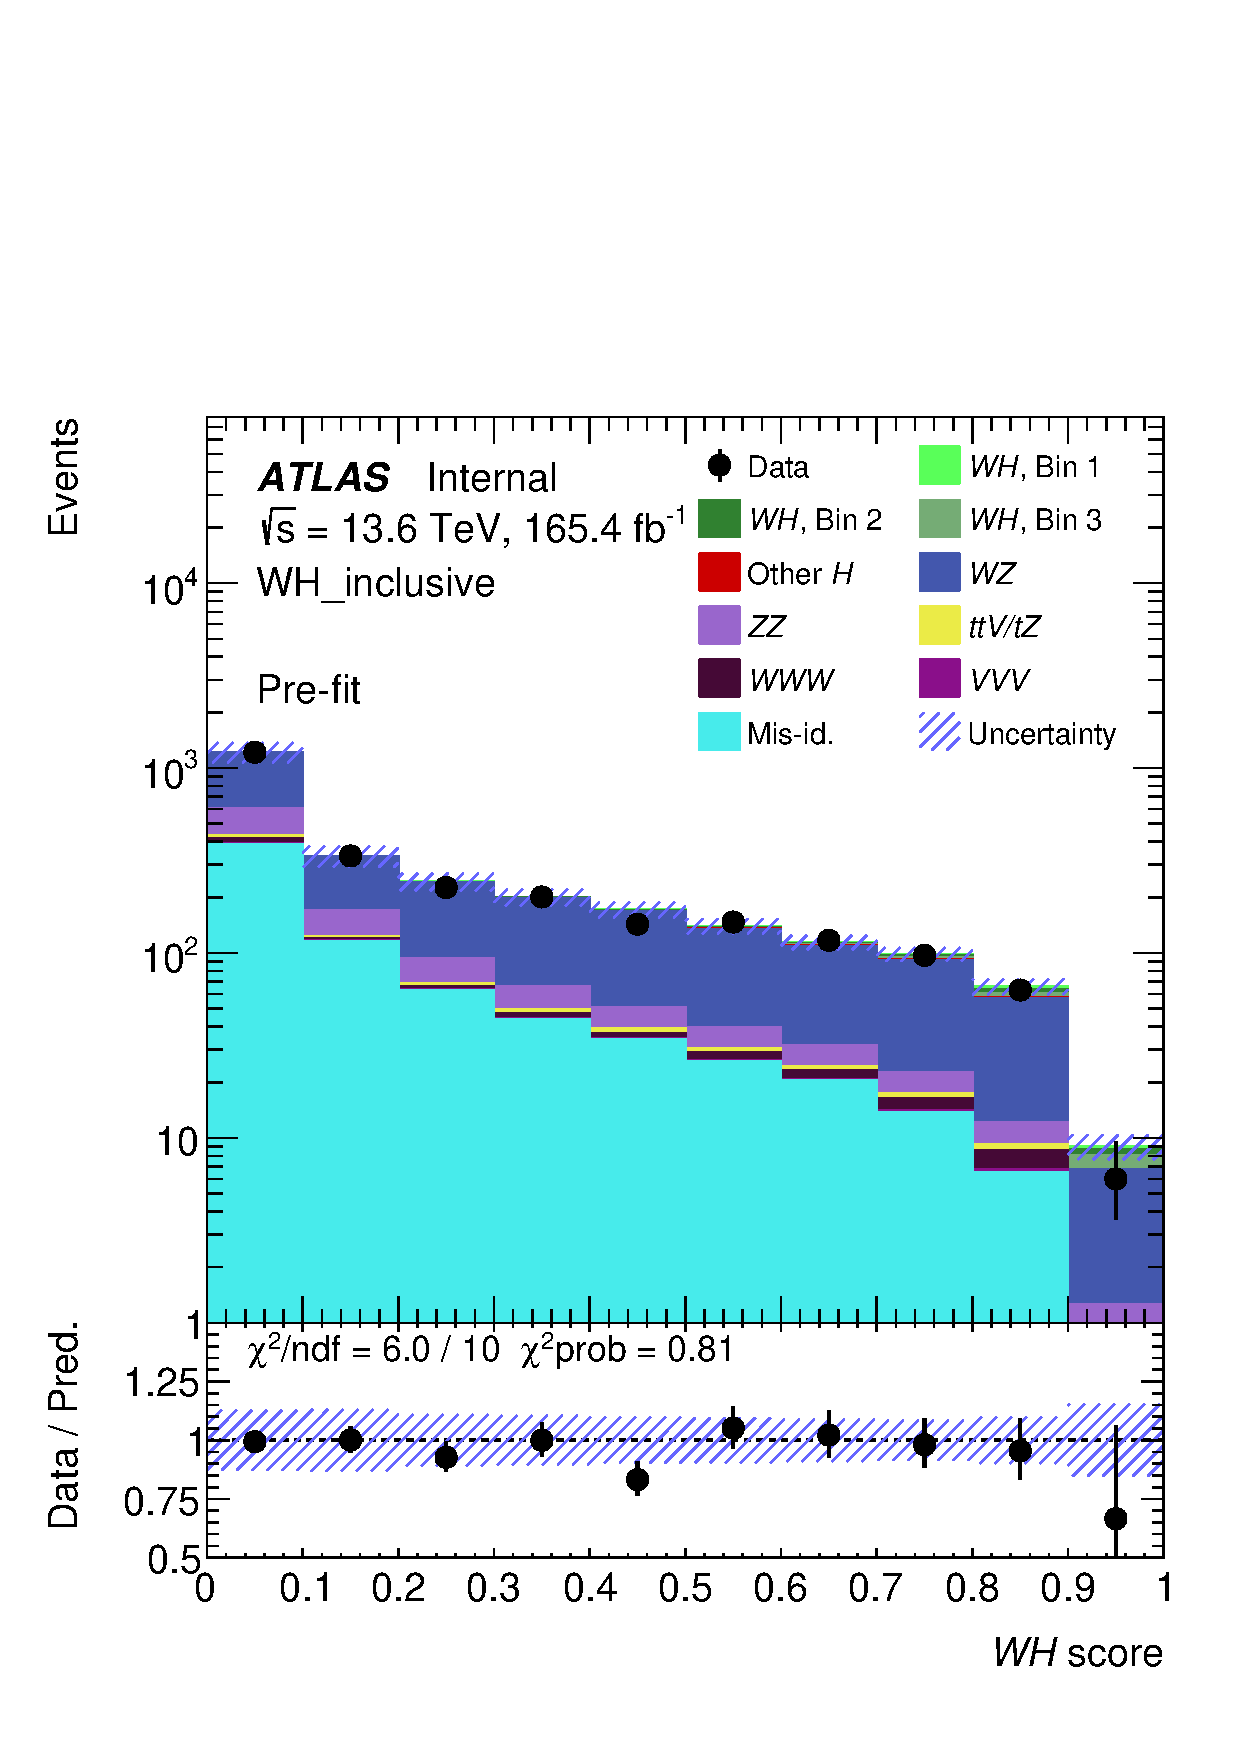
\includegraphics[width=0.4\textwidth]{figures/VH/VH_zdom_wh_scores.pdf}\label{fig:vh_wh_zdom_wh_outputs}
  }
  \subfloat[\zdom{} $WZ$ output node score]{
    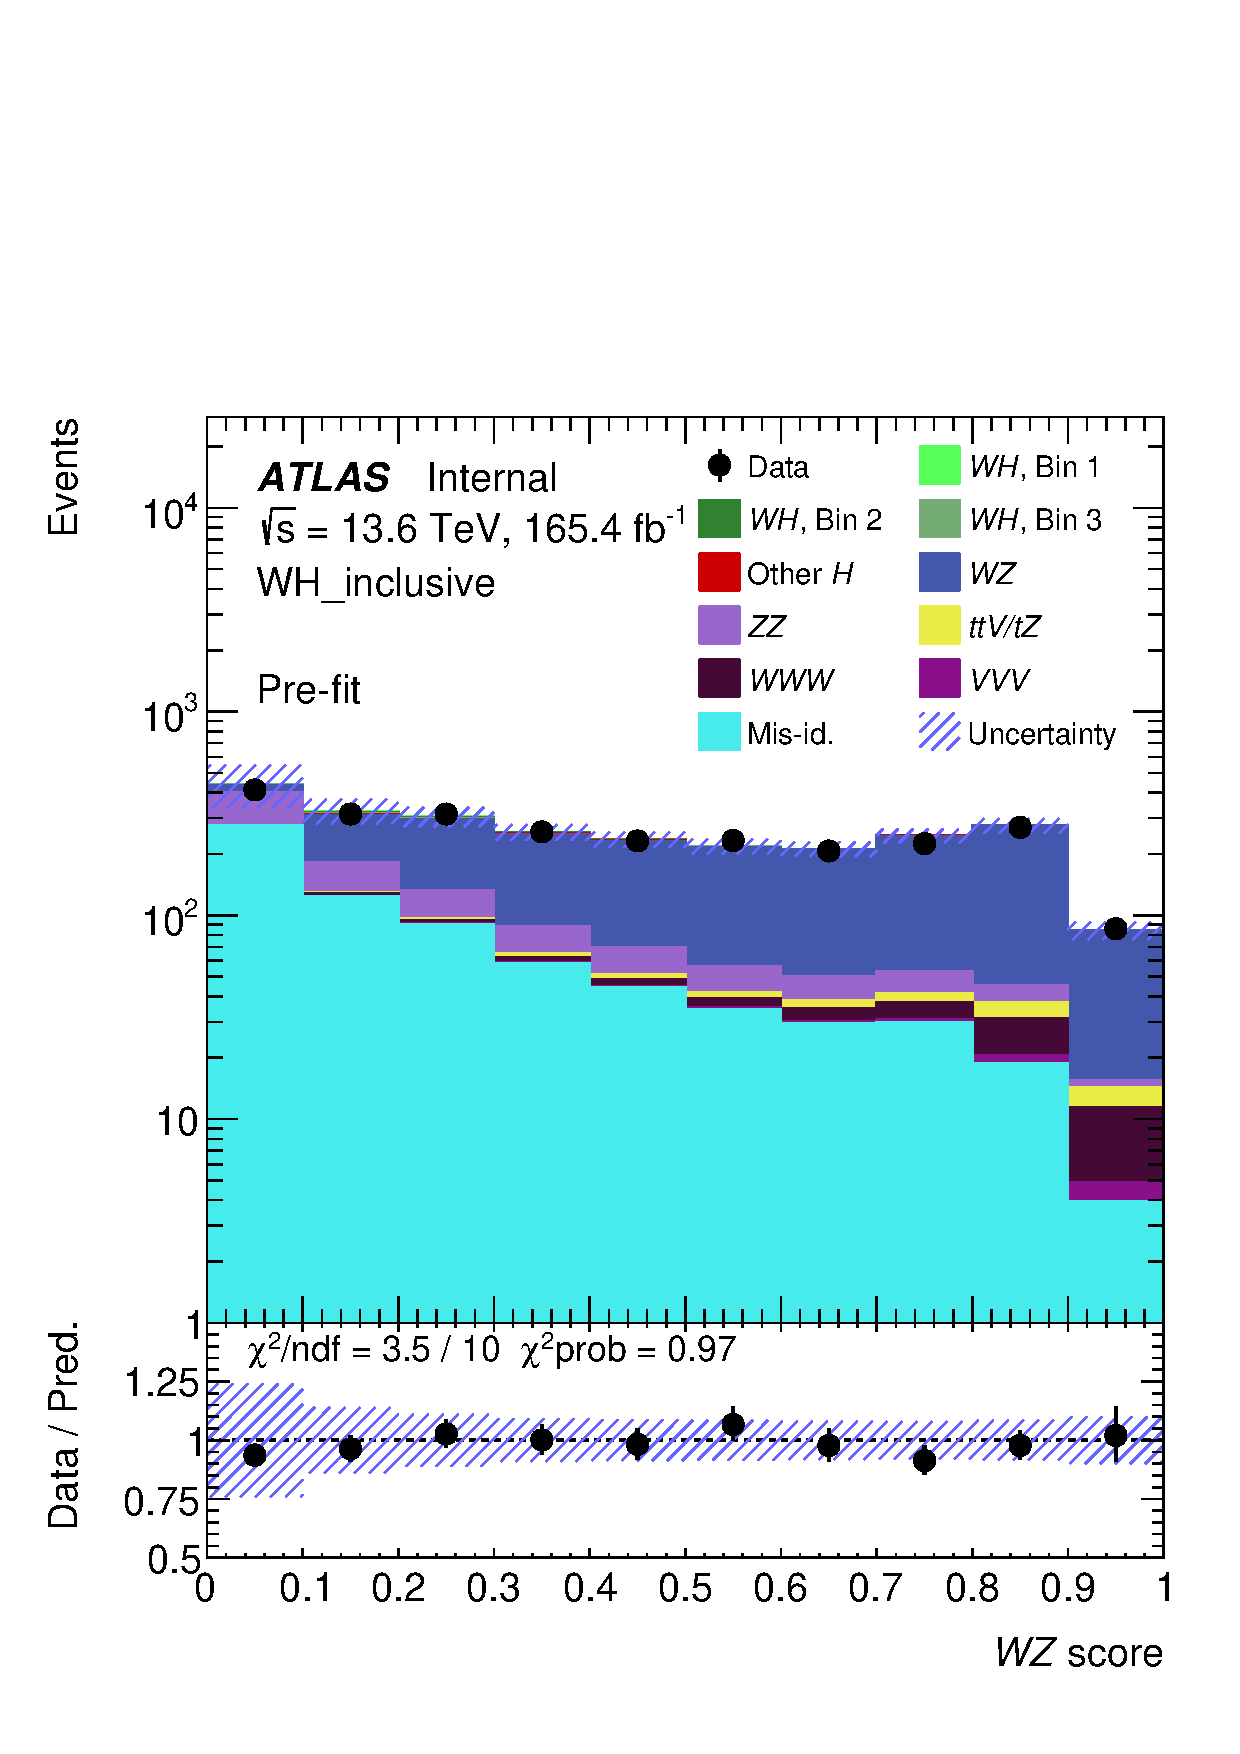
\includegraphics[width=0.4\textwidth]{figures/VH/VH_zdom_wz_scores.pdf}\label{fig:vh_wh_zdom_wz_outputs}
  }
  \hfill
  \subfloat[\zdom{} $ZZ$ output node score]{
    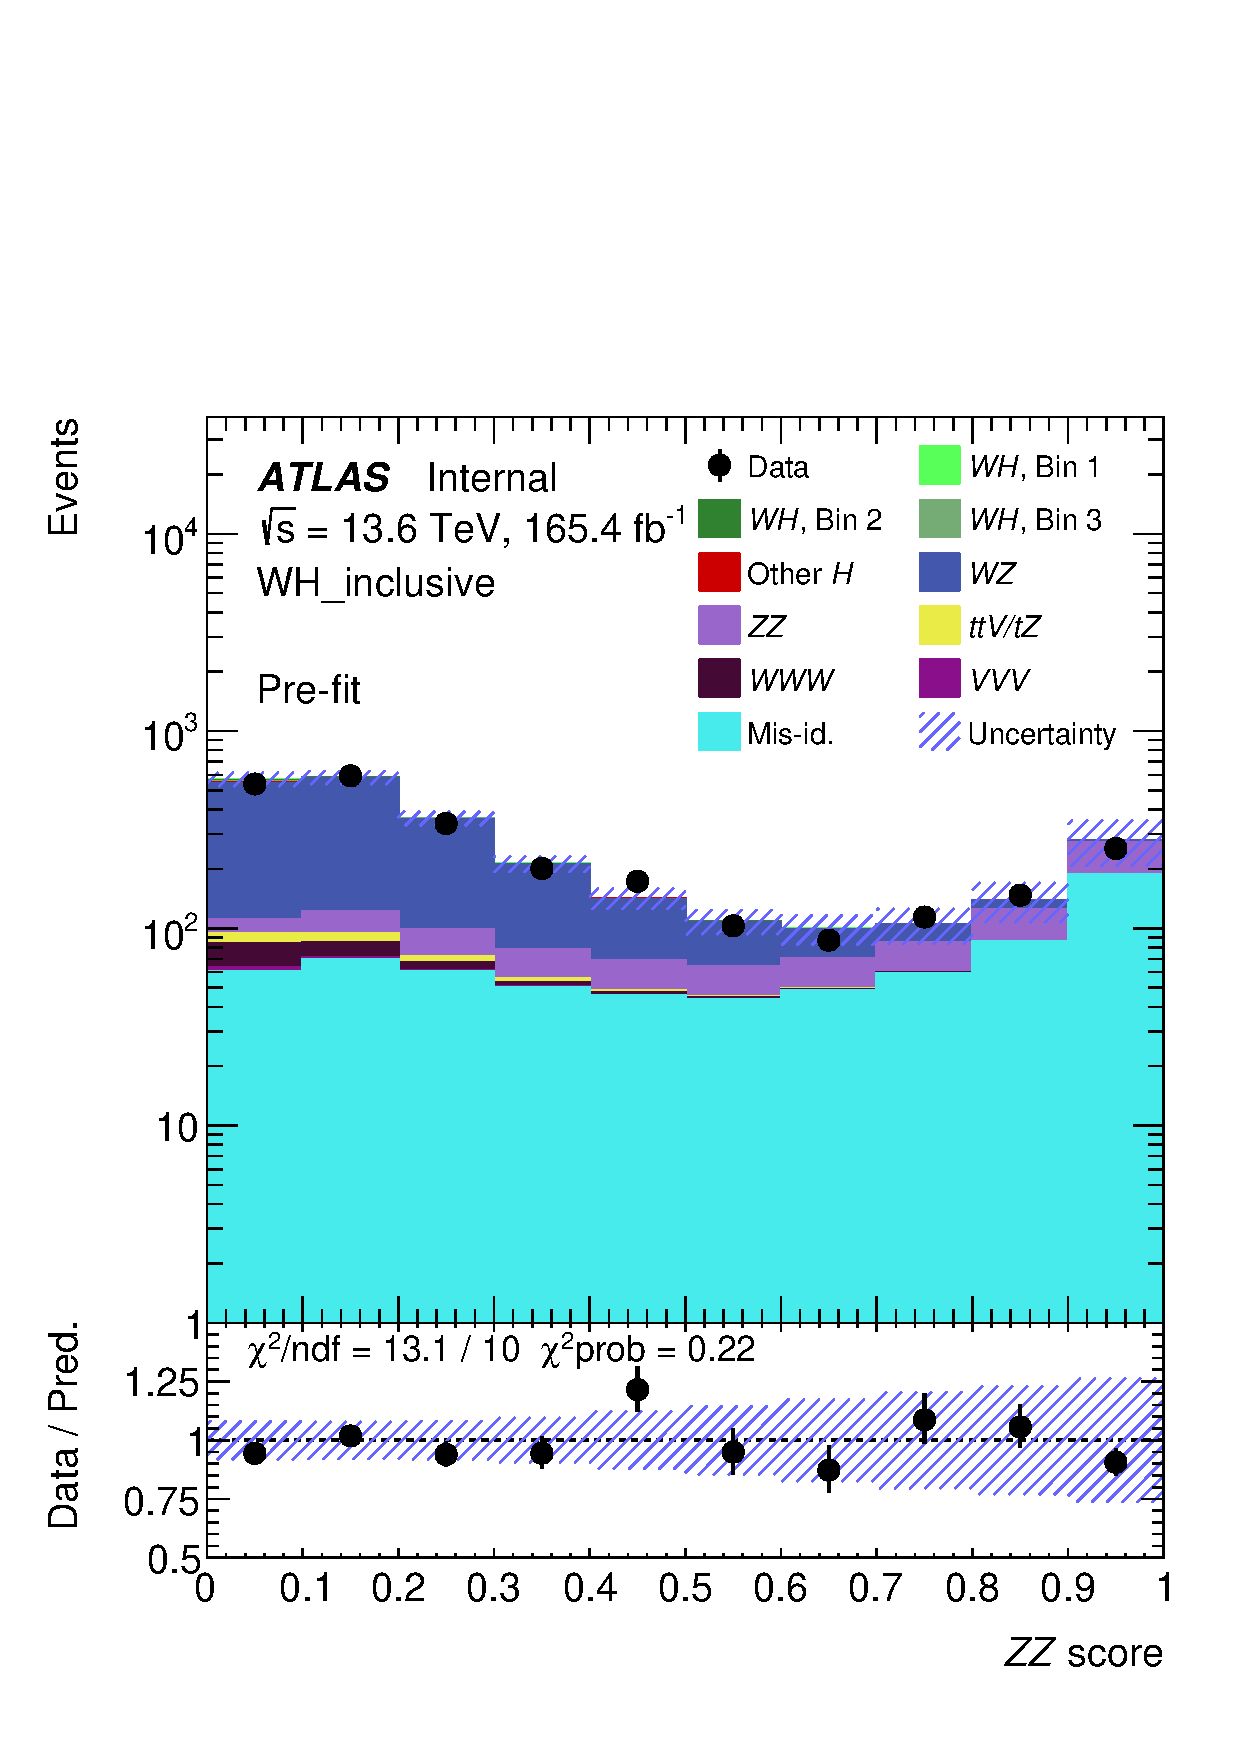
\includegraphics[width=0.4\textwidth]{figures/VH/VH_zdom_zz_scores.pdf}\label{fig:vh_wh_zdom_zz_outputs}
  }
  \caption{ANN outputs for the \zdom{} SR\@. The $WH$, $WZ$, and $ZZ$ output node scores are shown in (a), (b), and (c), respectively. The \wh{} Bins~1--3 correspond to the STXS bins of the \wh{} process, with Bin~1 defined as $\ptv{} < 75$~GeV, Bin~2 as $75 \leq \ptv{} < 150$~GeV, and Bin~3 as $\ptv{} \geq 150$~GeV.}\label{fig:vh_wh_zdom_outputs}
\end{figure}

\begin{figure}[htp]
  \centering
  \subfloat[\zdom{} ANN discriminant for $\ptv{} < 75$~GeV]{
    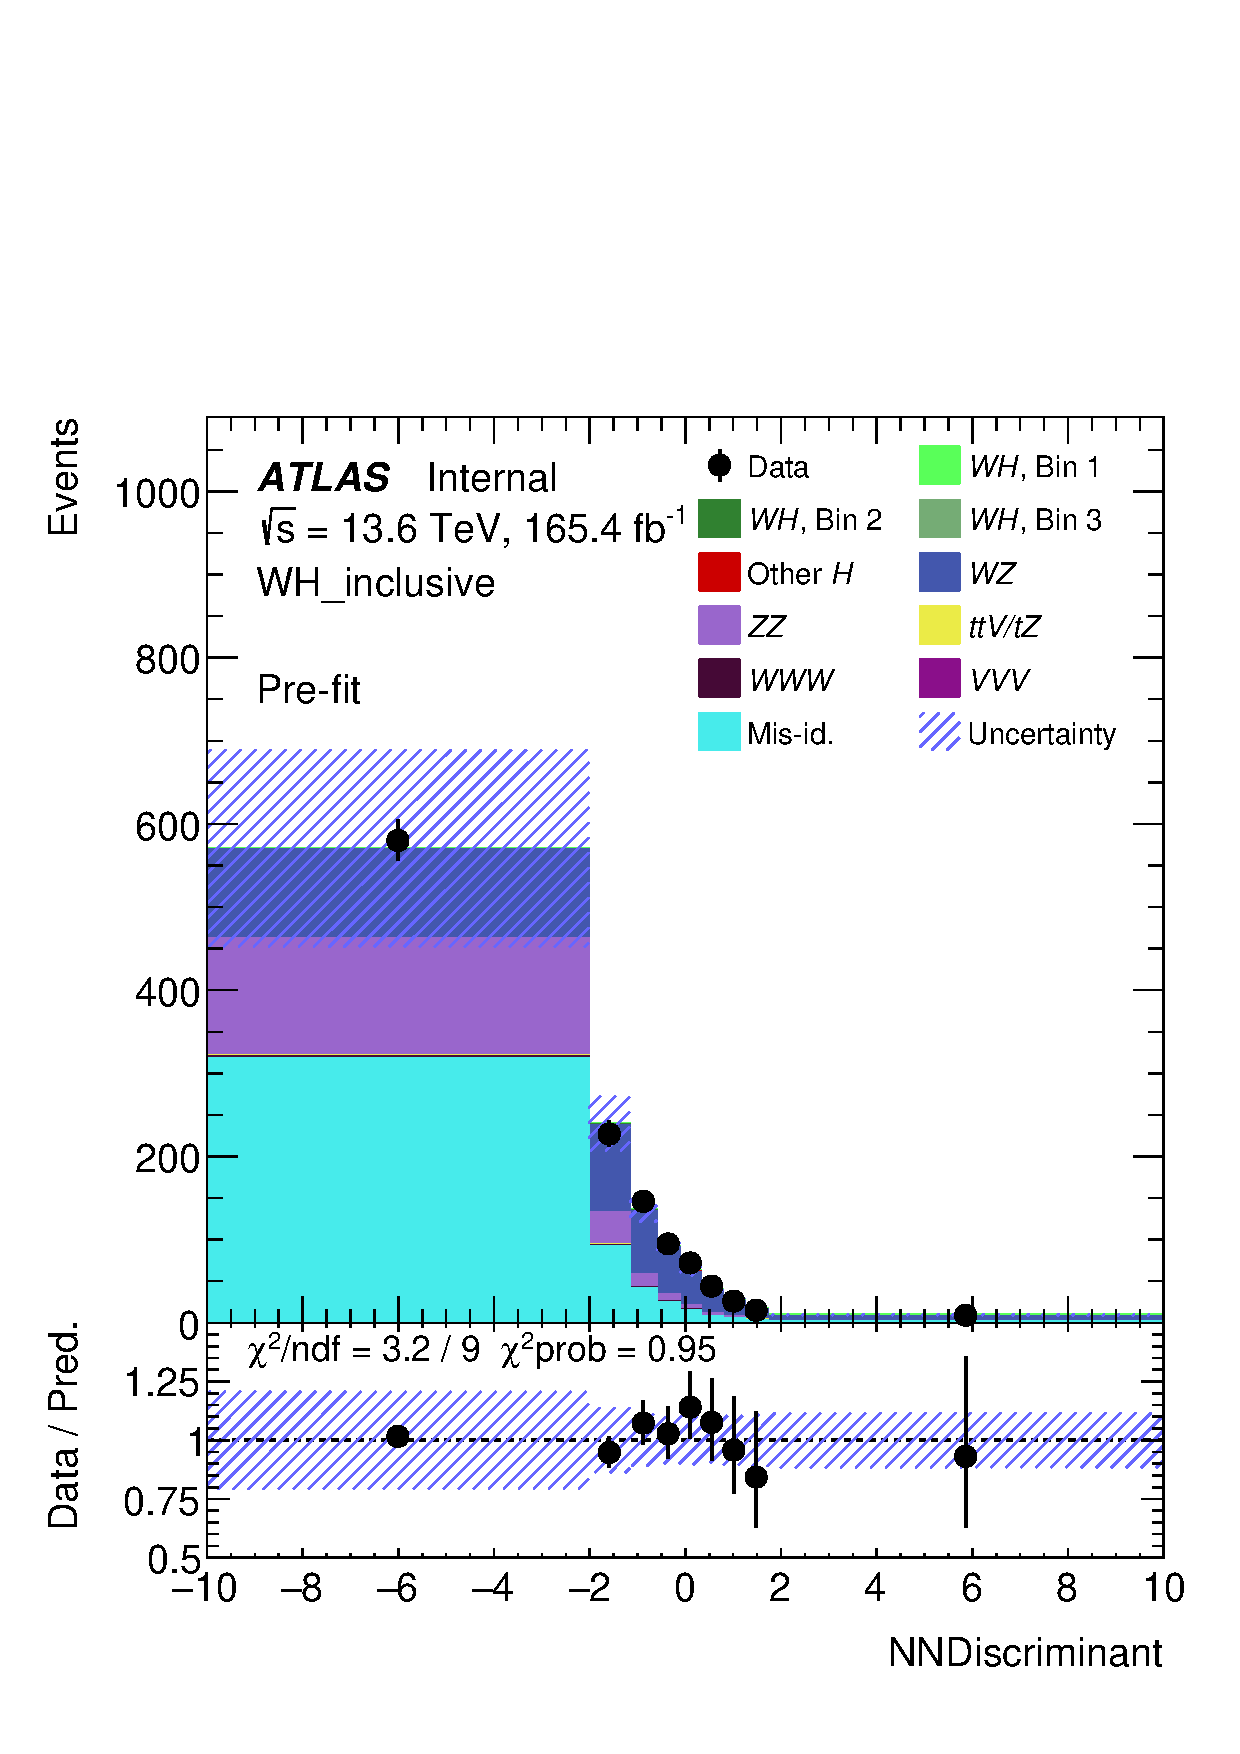
\includegraphics[width=0.4\textwidth]{figures/VH/VH_zdom_nn_discriminant_0to75.pdf}\label{fig:vh_wh_zdom_wh_discriminant_0to75}
  }
  \subfloat[\zdom{} ANN discriminant for $75 \leq \ptv{} < 150$~GeV]{
    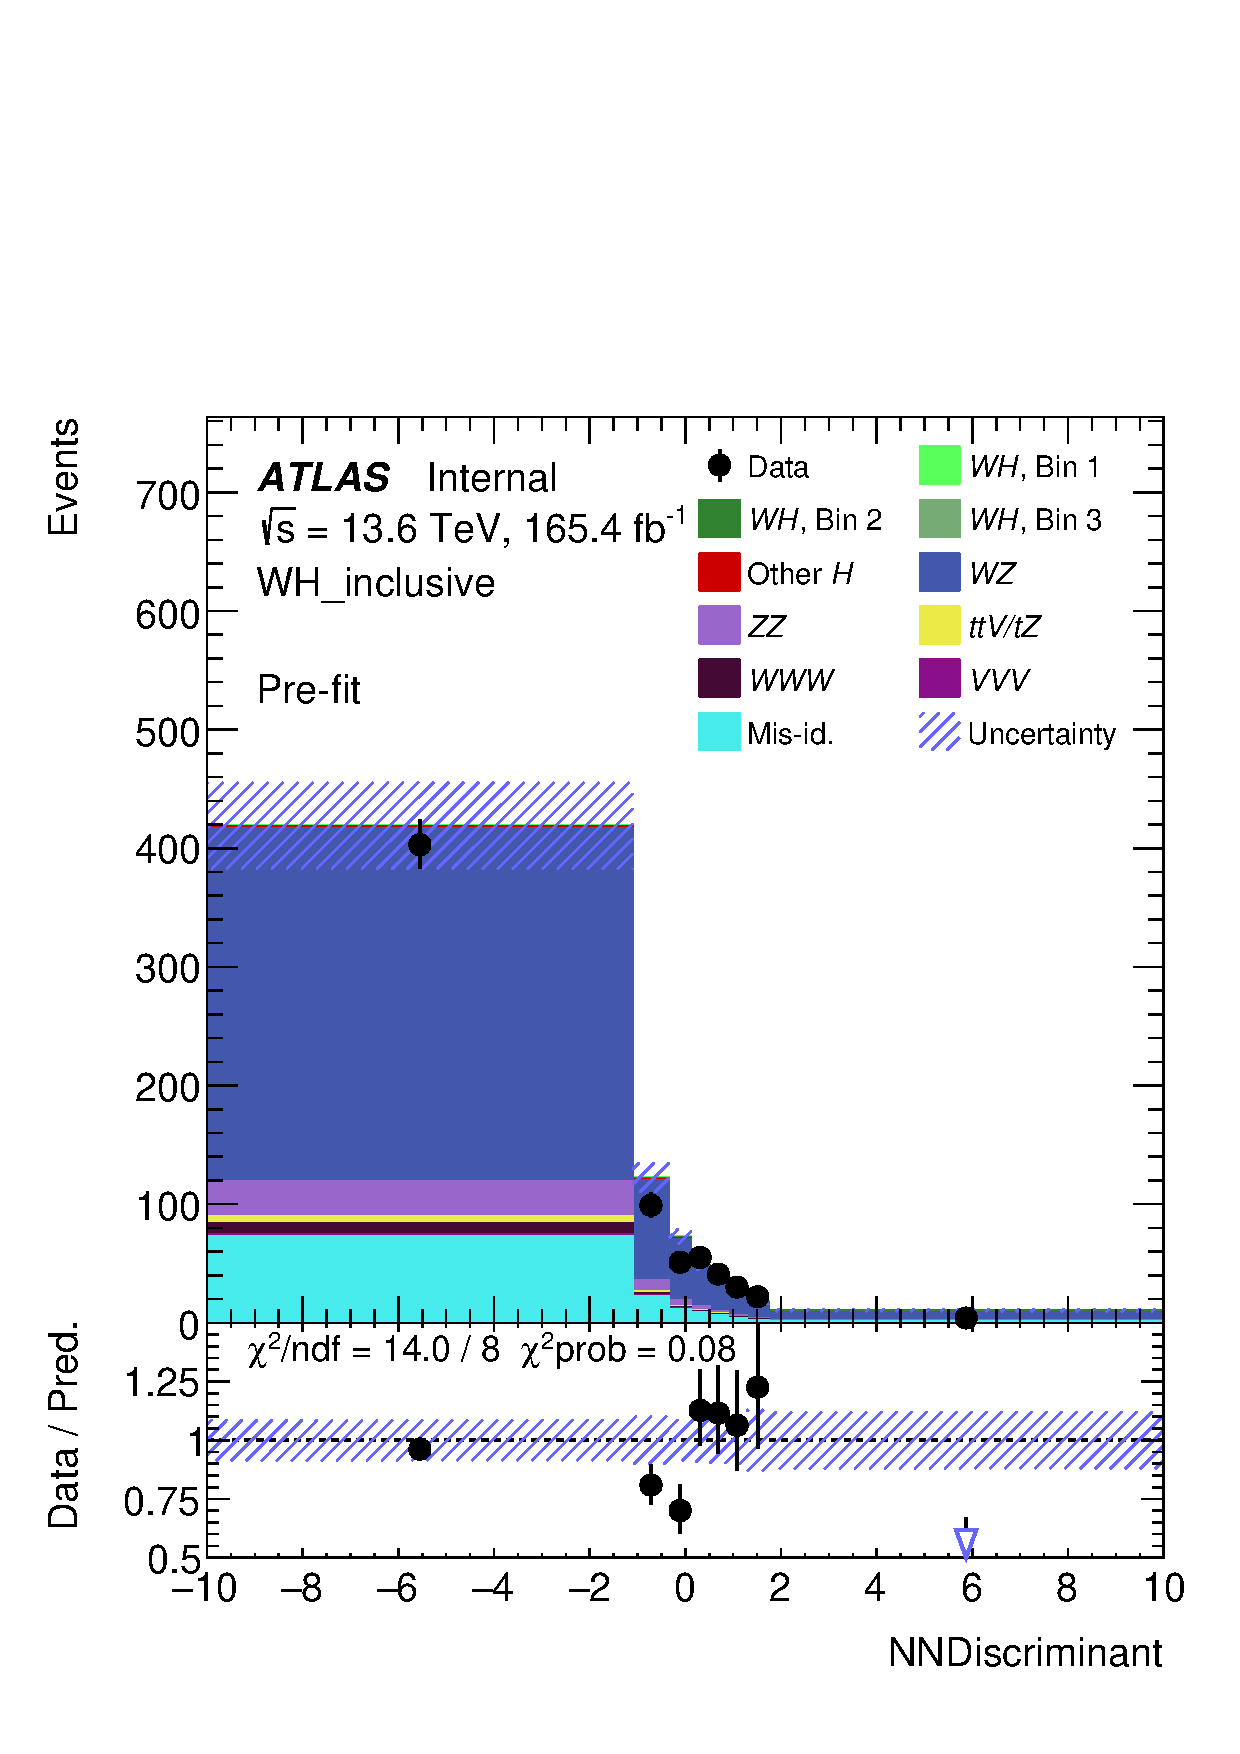
\includegraphics[width=0.4\textwidth]{figures/VH/VH_zdom_nn_discriminant_75to150.pdf}\label{fig:vh_wh_zdom_wz_discriminant_75to150}
  }
  \hfill
  \subfloat[\zdom{} ANN discriminant for $\ptv{} \geq 150$~GeV]{
    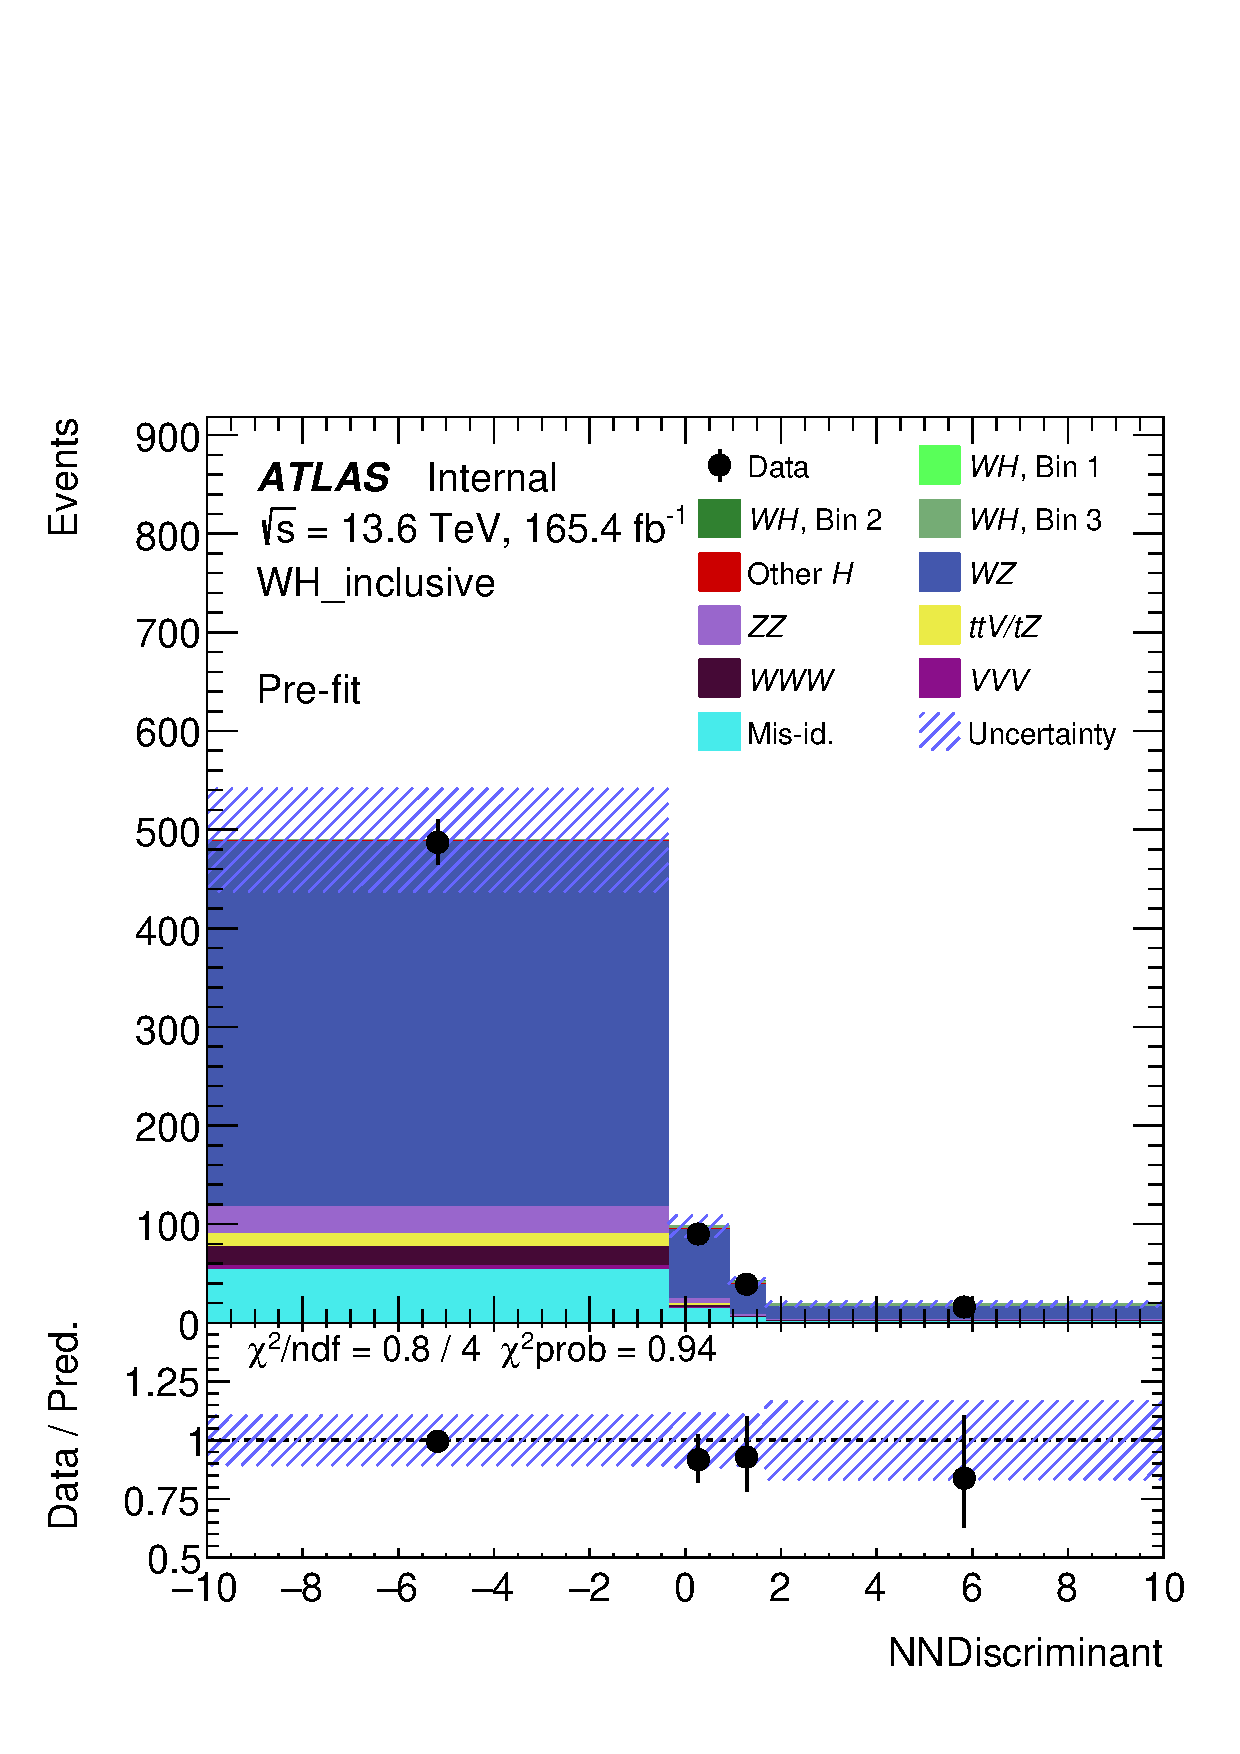
\includegraphics[width=0.4\textwidth]{figures/VH/VH_zdom_nn_discriminant_150toinf.pdf}\label{fig:vh_wh_zdom_zz_discriminant_150toinf}
  }
  \caption{ANN discriminant for the \zdom{} SR split by the transverse momentum of the associated $W$ boson.}\label{fig:vh_wh_zdom_discriminant}
\end{figure}

\begin{figure}[htp]
  \centering
  \subfloat[\zdep{} $WH$ output node score]{
    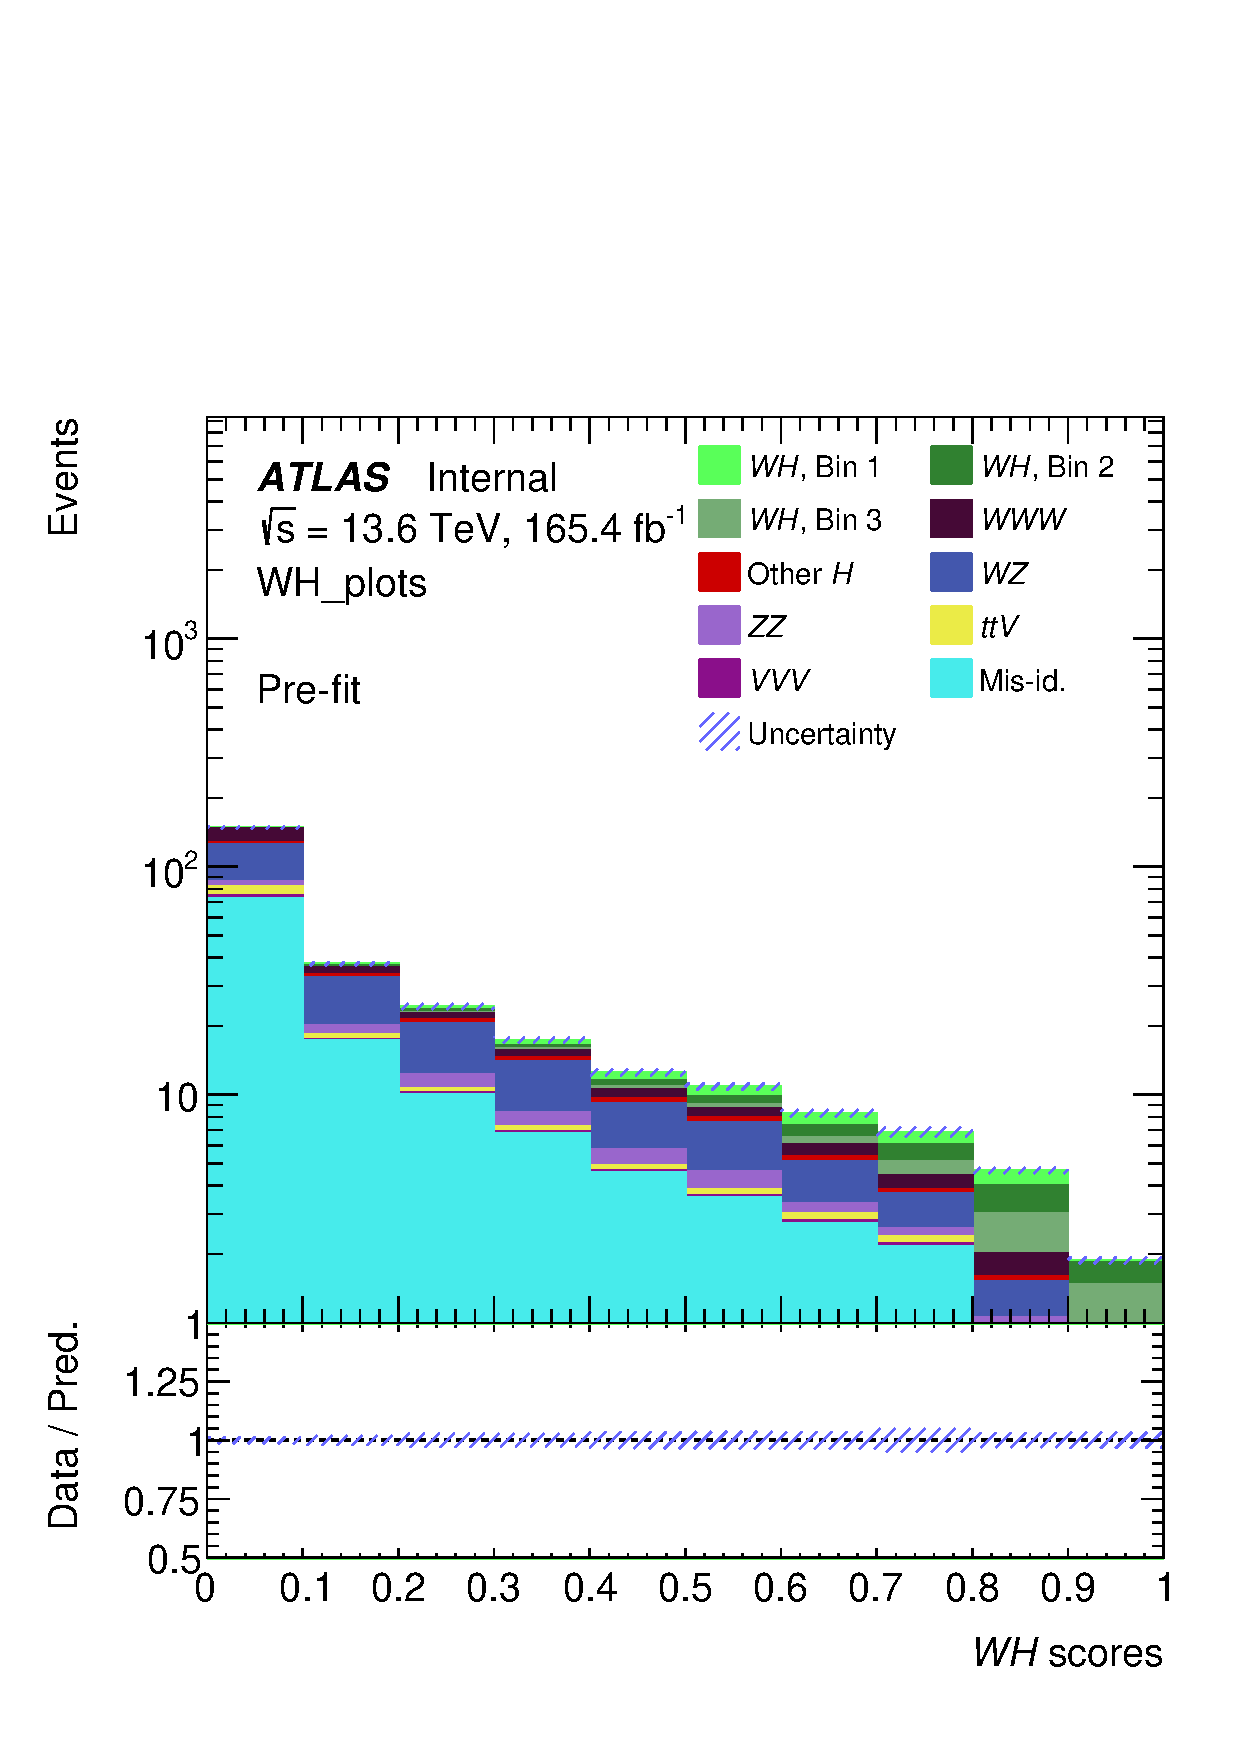
\includegraphics[width=0.4\textwidth]{figures/VH/VH_zdep_wh_scores.pdf}\label{fig:vh_wh_zdep_wh_outputs}
  }
  \subfloat[\zdep{} $WZ$ output node score]{
    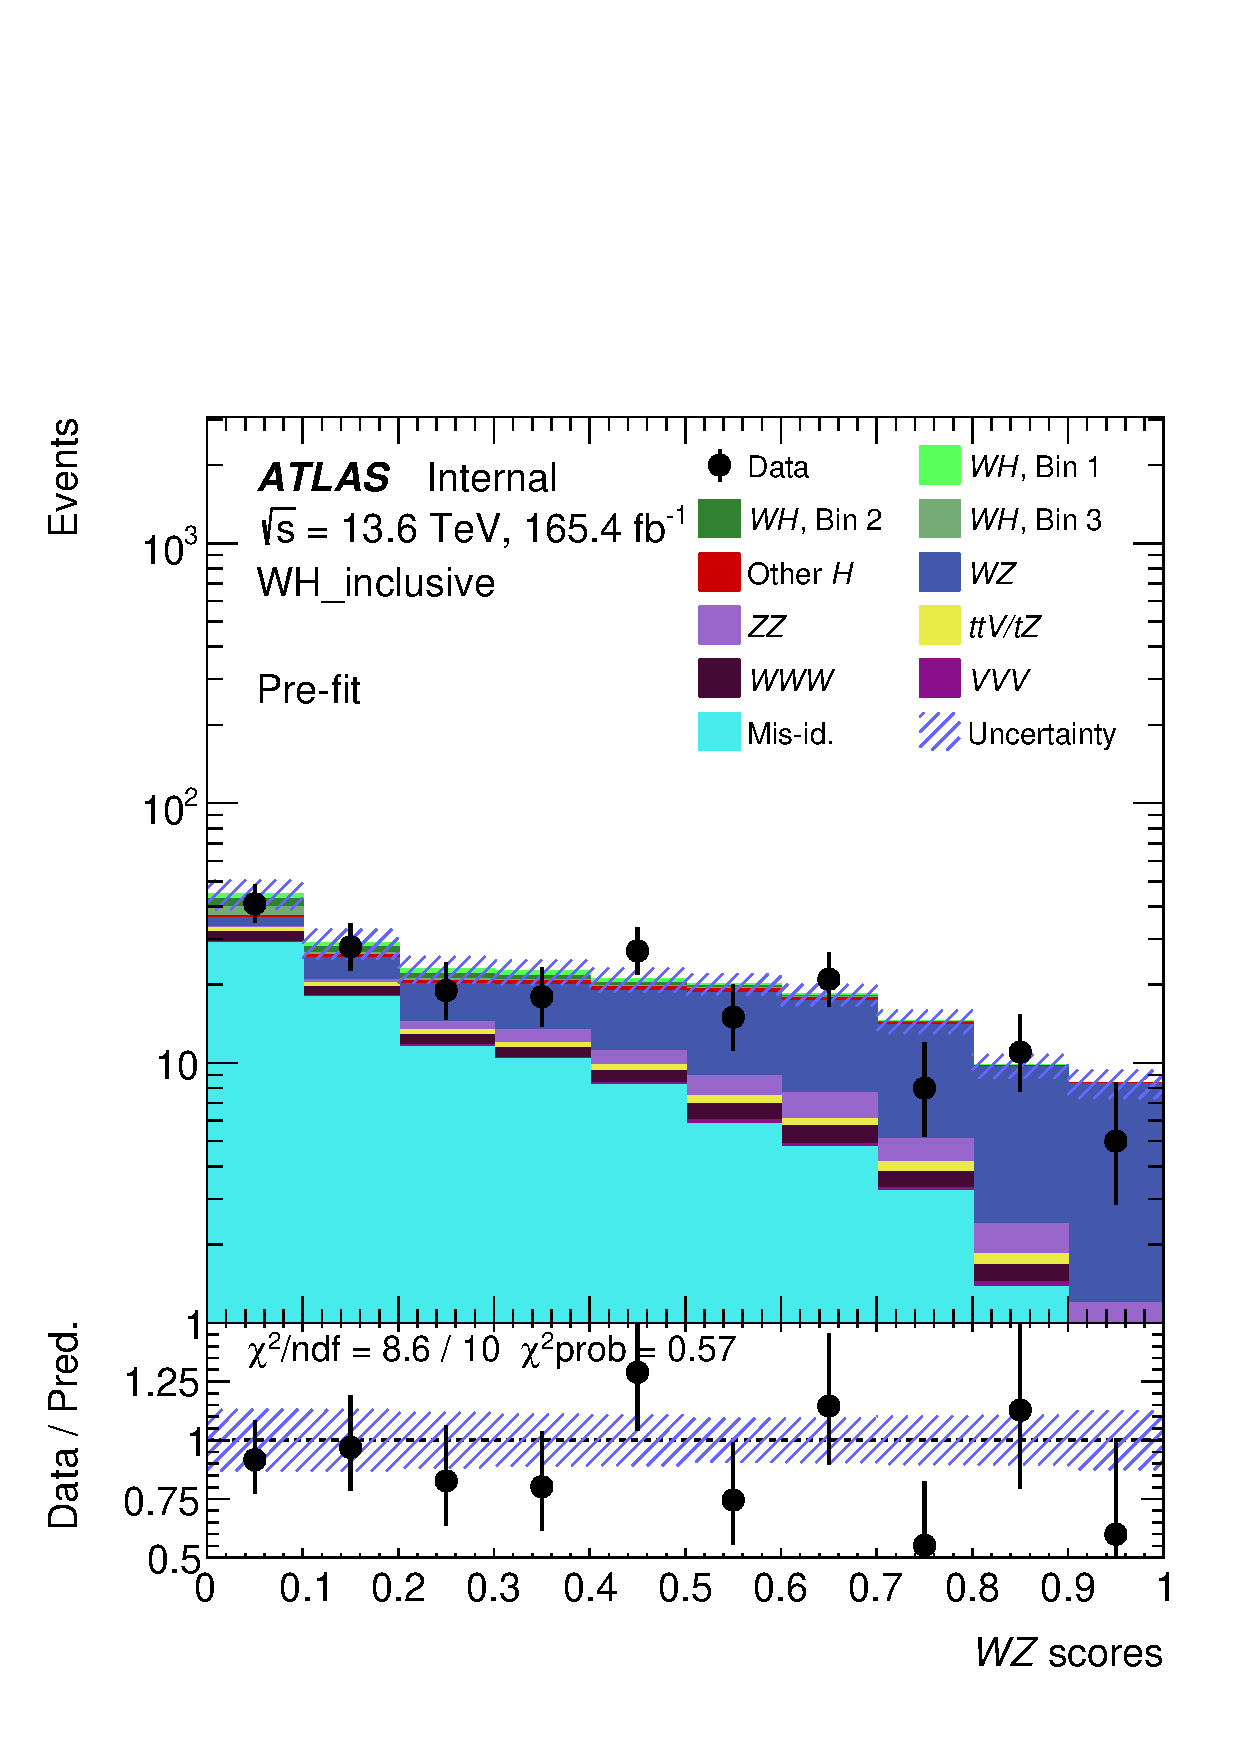
\includegraphics[width=0.4\textwidth]{figures/VH/VH_zdep_wz_scores.pdf}\label{fig:vh_wh_zdep_wz_outputs}
  }
  \hfill
  \subfloat[\zdep{} $WWW$ output node score]{
    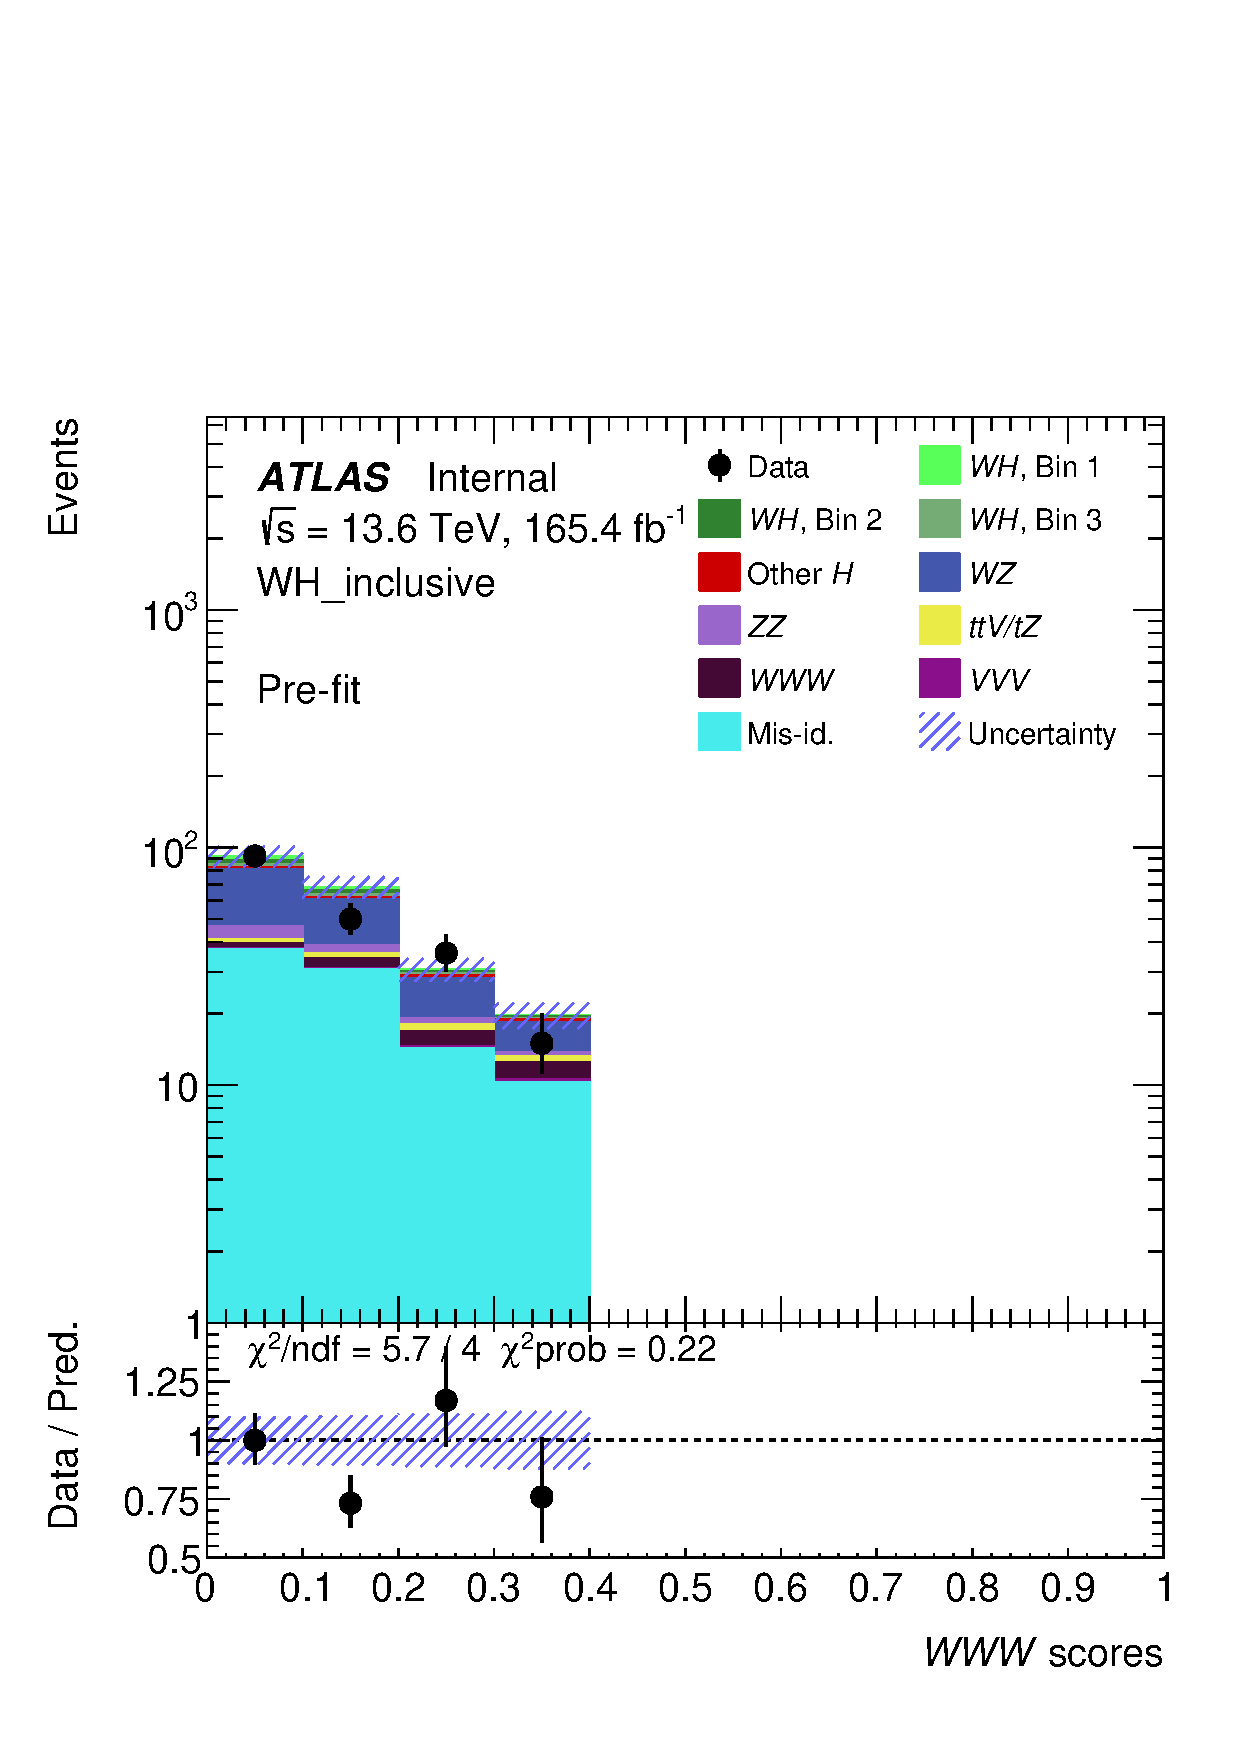
\includegraphics[width=0.4\textwidth]{figures/VH/VH_zdep_www_scores.pdf}\label{fig:vh_wh_zdep_www_outputs}
  }
  \subfloat[\zdep{} $t\bar{t}$ output node score]{
    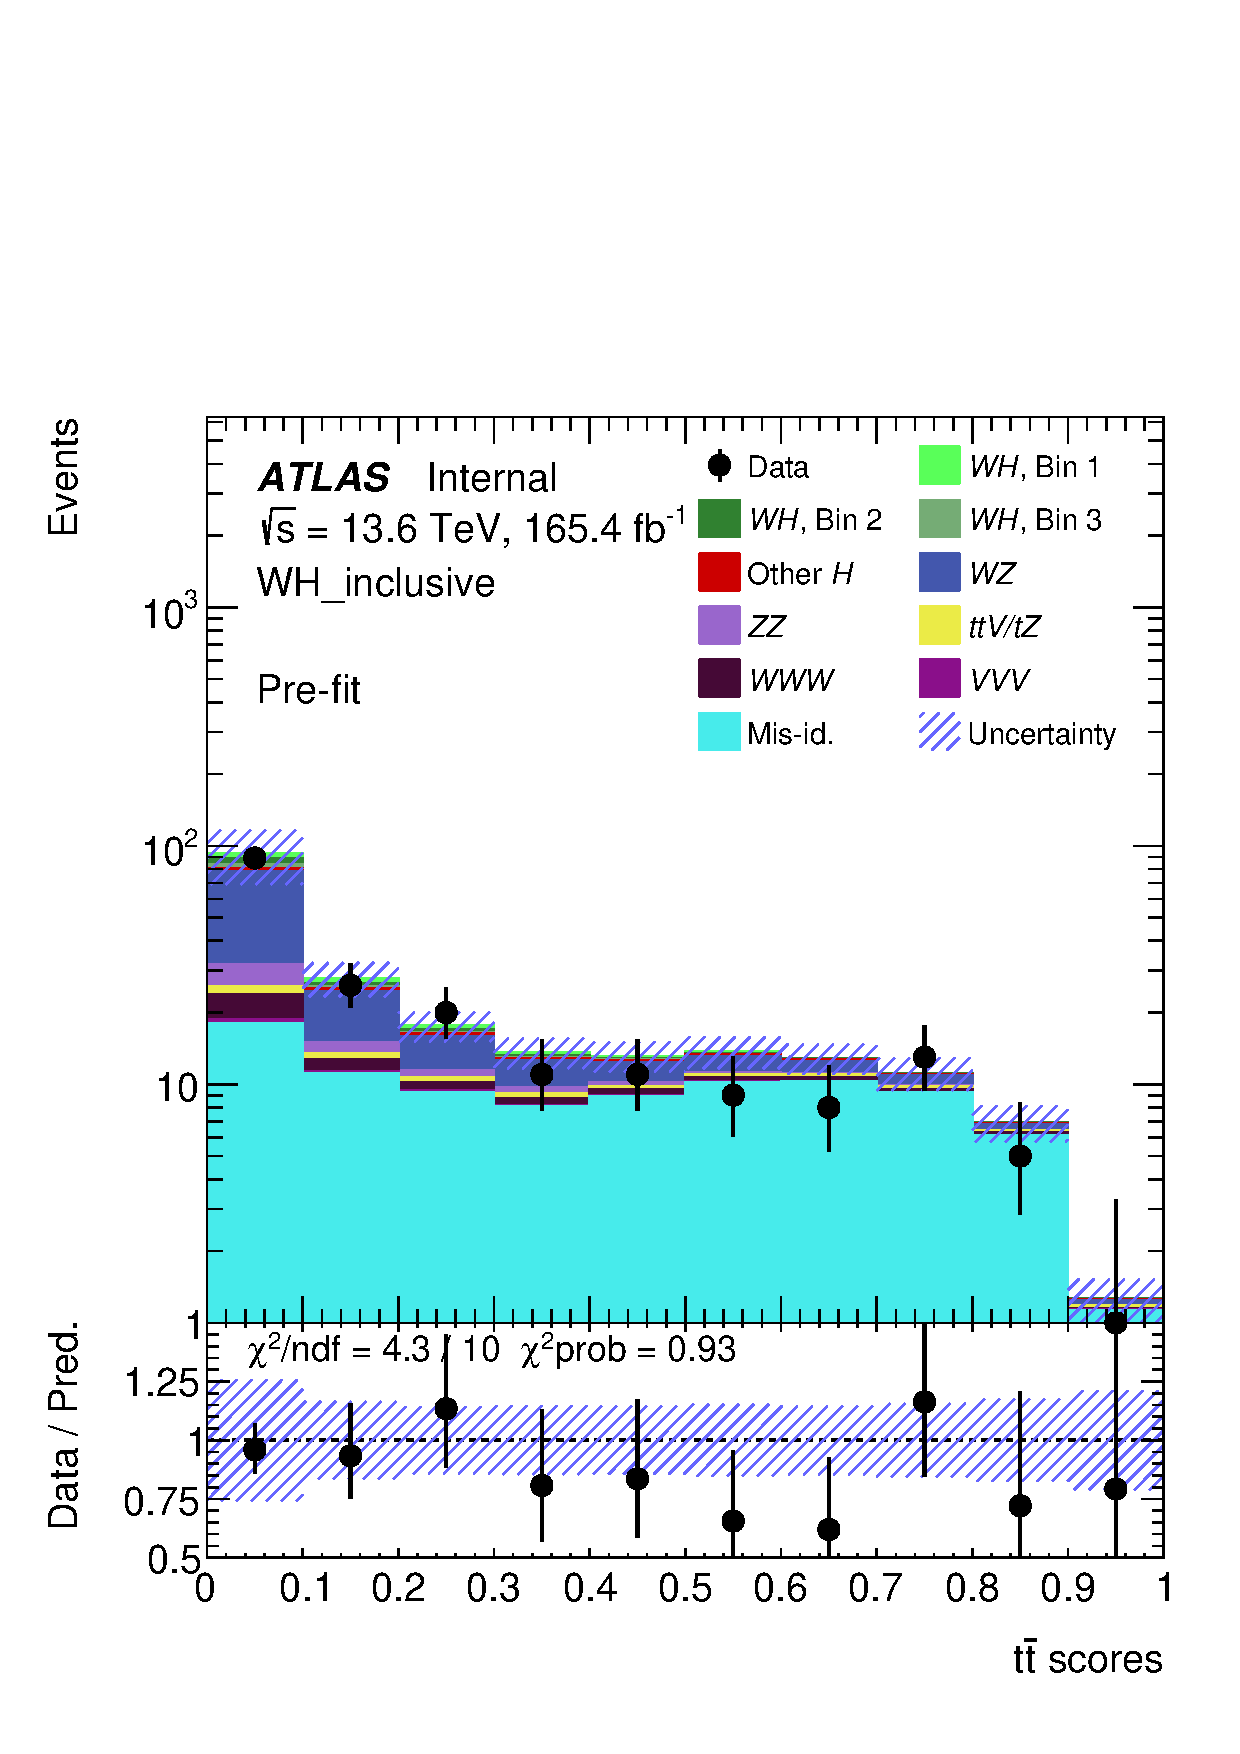
\includegraphics[width=0.4\textwidth]{figures/VH/VH_zdep_ttbar_scores.pdf}\label{fig:vh_wh_zdep_ttbar_outputs}
  }
  \caption{ANN outputs for the \zdep{} SR\@. The $WH$, $WZ$, $WWW$, and $t\bar{t}$ output node scores are shown in (a), (b), (c) and (d), respectively.}\label{fig:vh_wh_zdep_outputs}
\end{figure}

\begin{figure}[htp]
  \centering
  \subfloat[\zdep{} ANN discriminant for $\ptv{} < 75$~GeV]{
    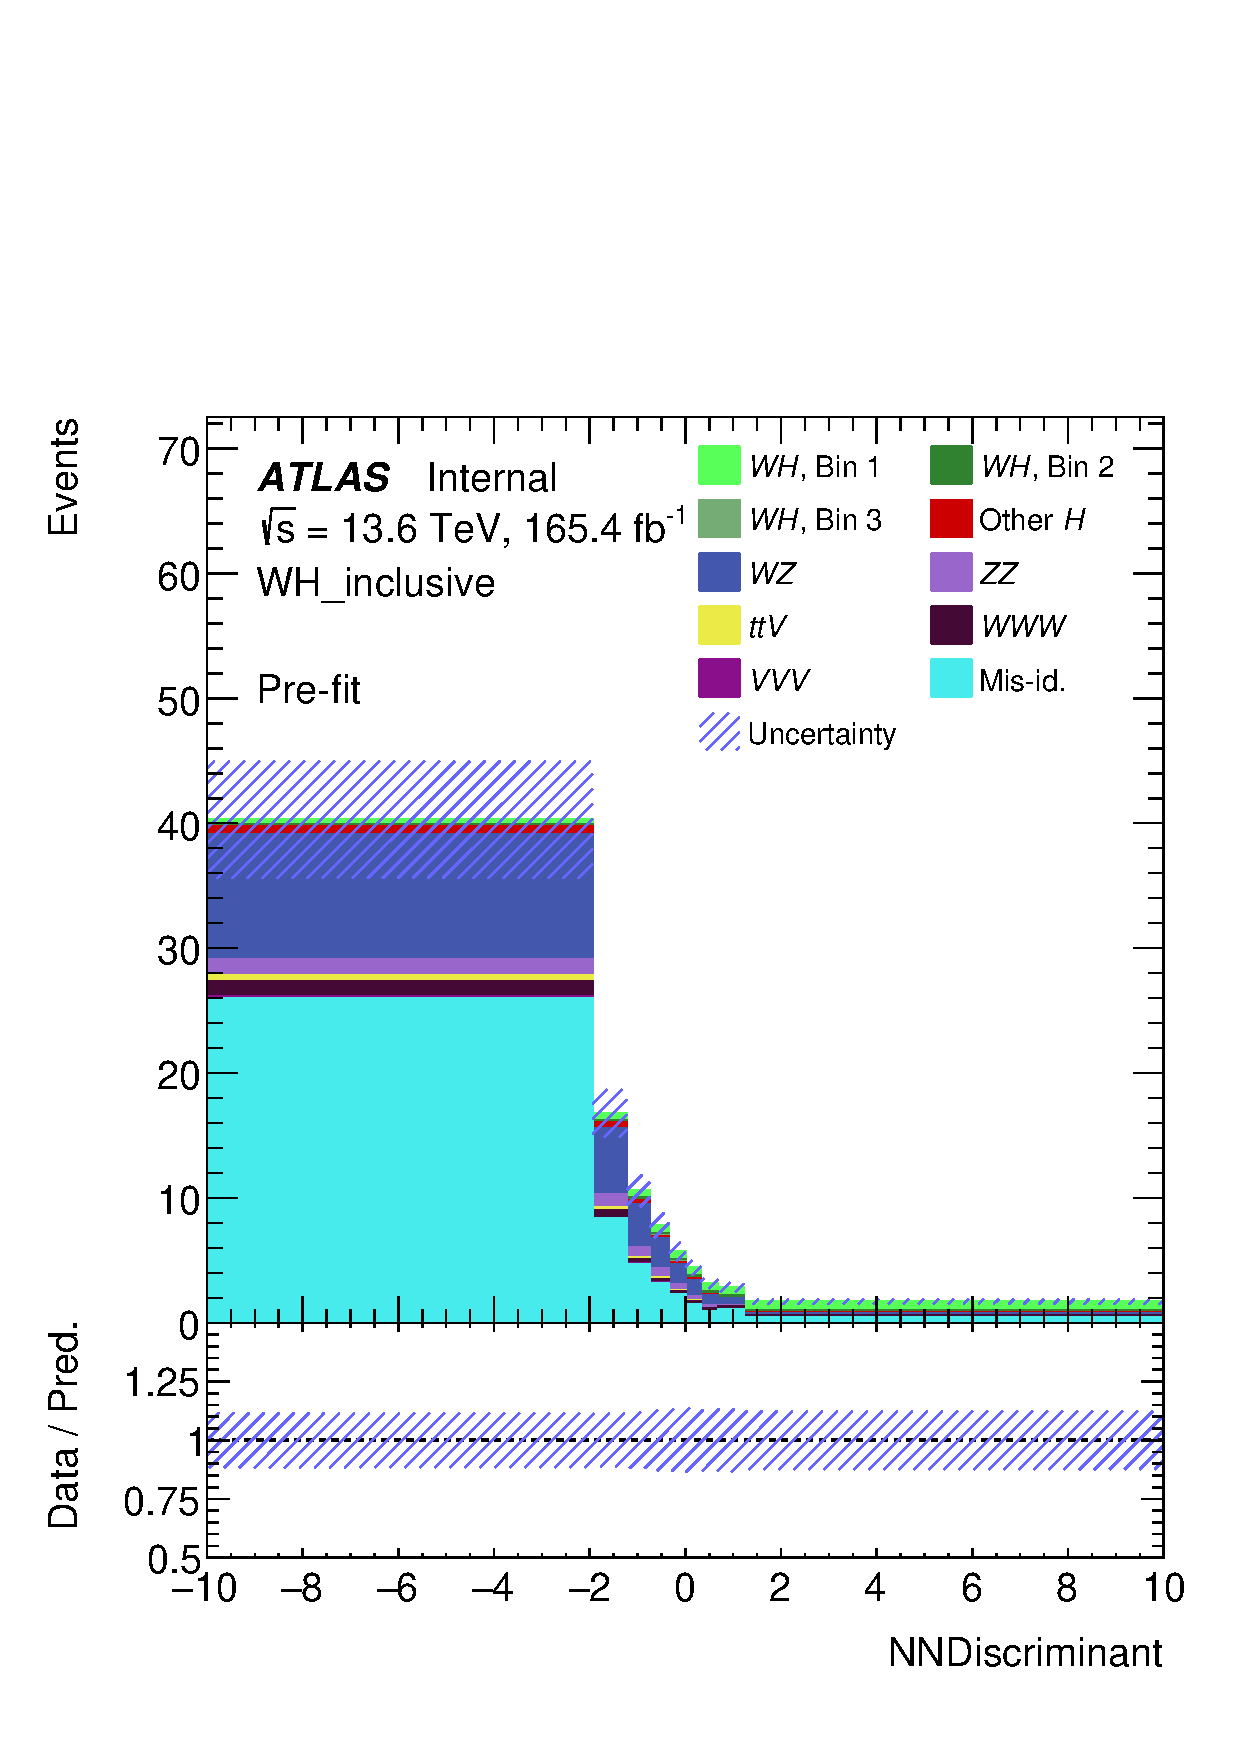
\includegraphics[width=0.4\textwidth]{figures/VH/VH_zdep_nn_discriminant_0to75.pdf}\label{fig:vh_wh_zdep_wh_discriminant_0to75}
  }
  \subfloat[\zdep{} ANN discriminant for $75 \leq \ptv{} < 150$~GeV]{
    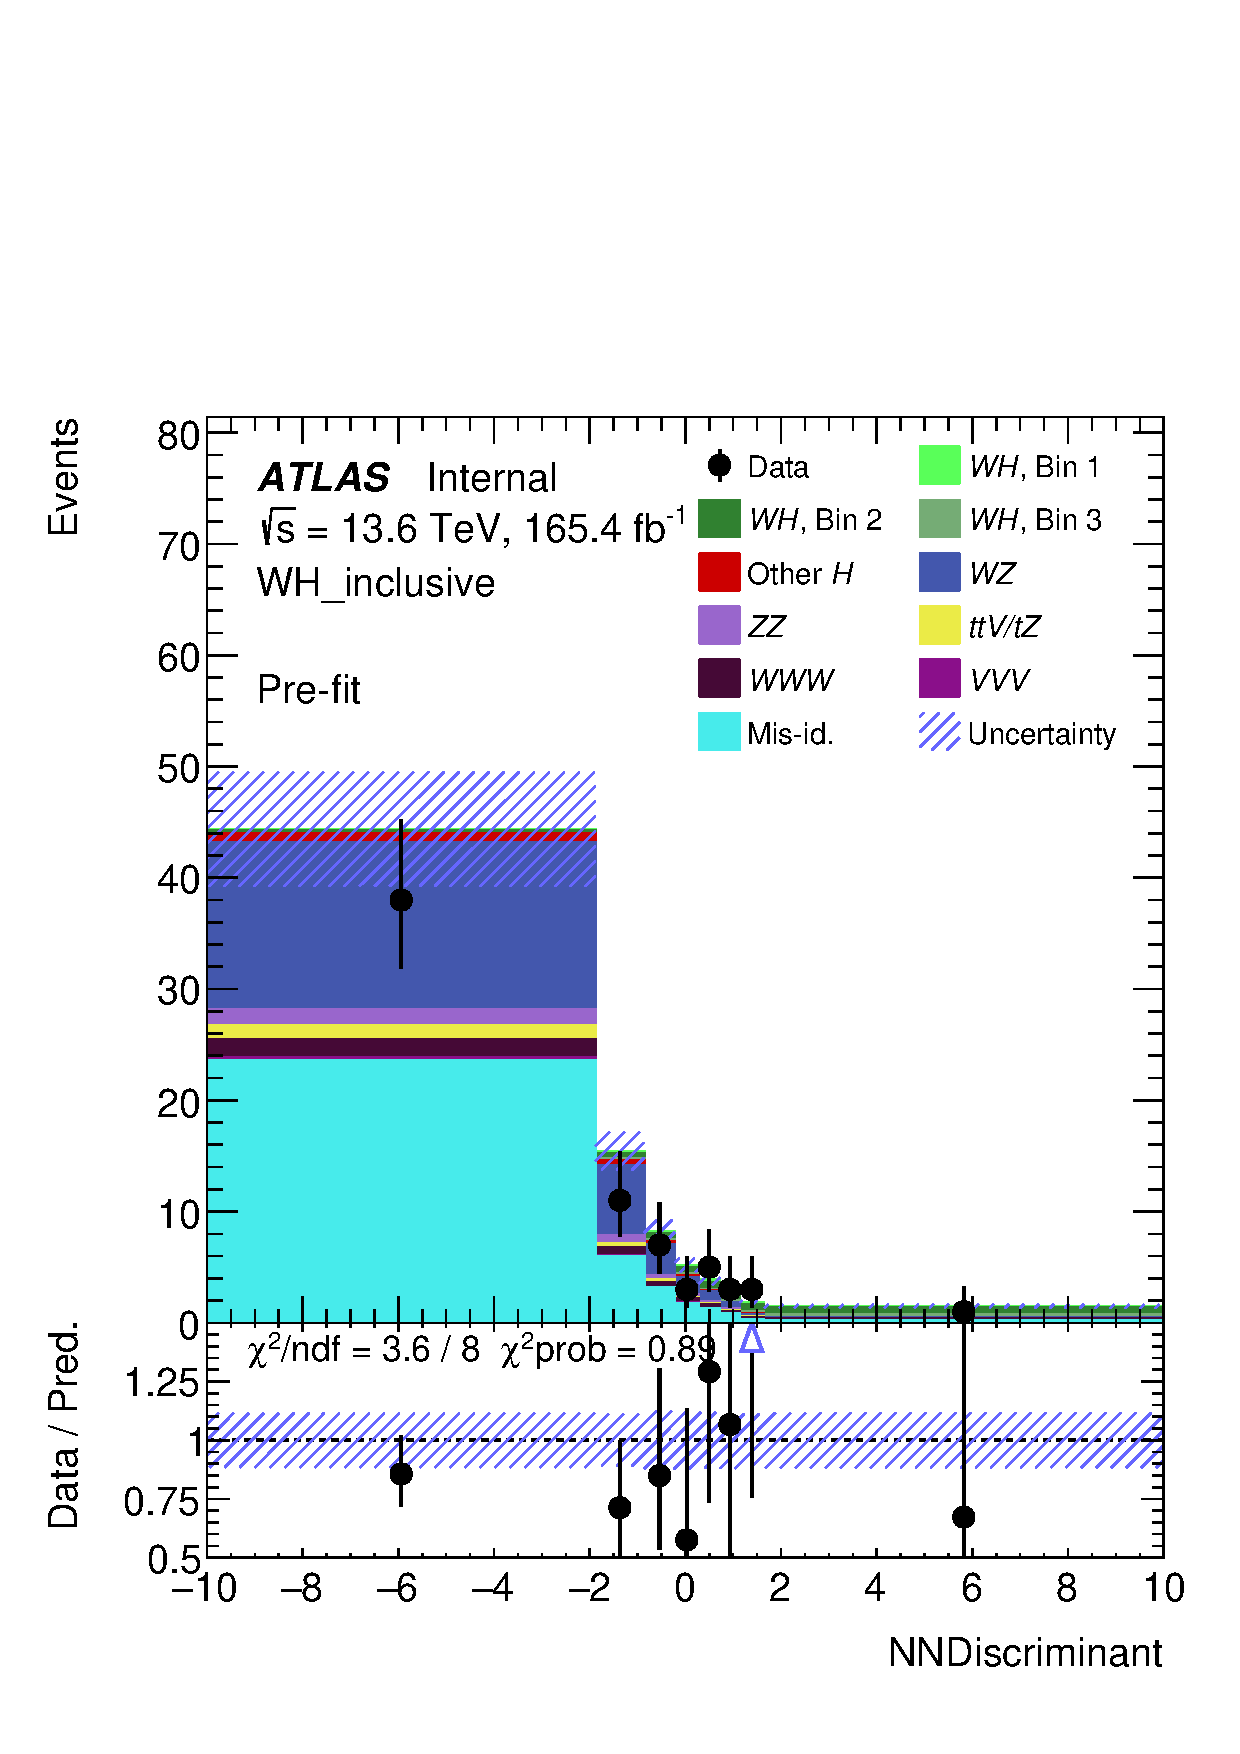
\includegraphics[width=0.4\textwidth]{figures/VH/VH_zdep_nn_discriminant_75to150.pdf}\label{fig:vh_wh_zdep_wz_discriminant_75to150}
  }
  \hfill
  \subfloat[\zdep{} ANN discriminant for $\ptv{} \geq 150$~GeV]{
    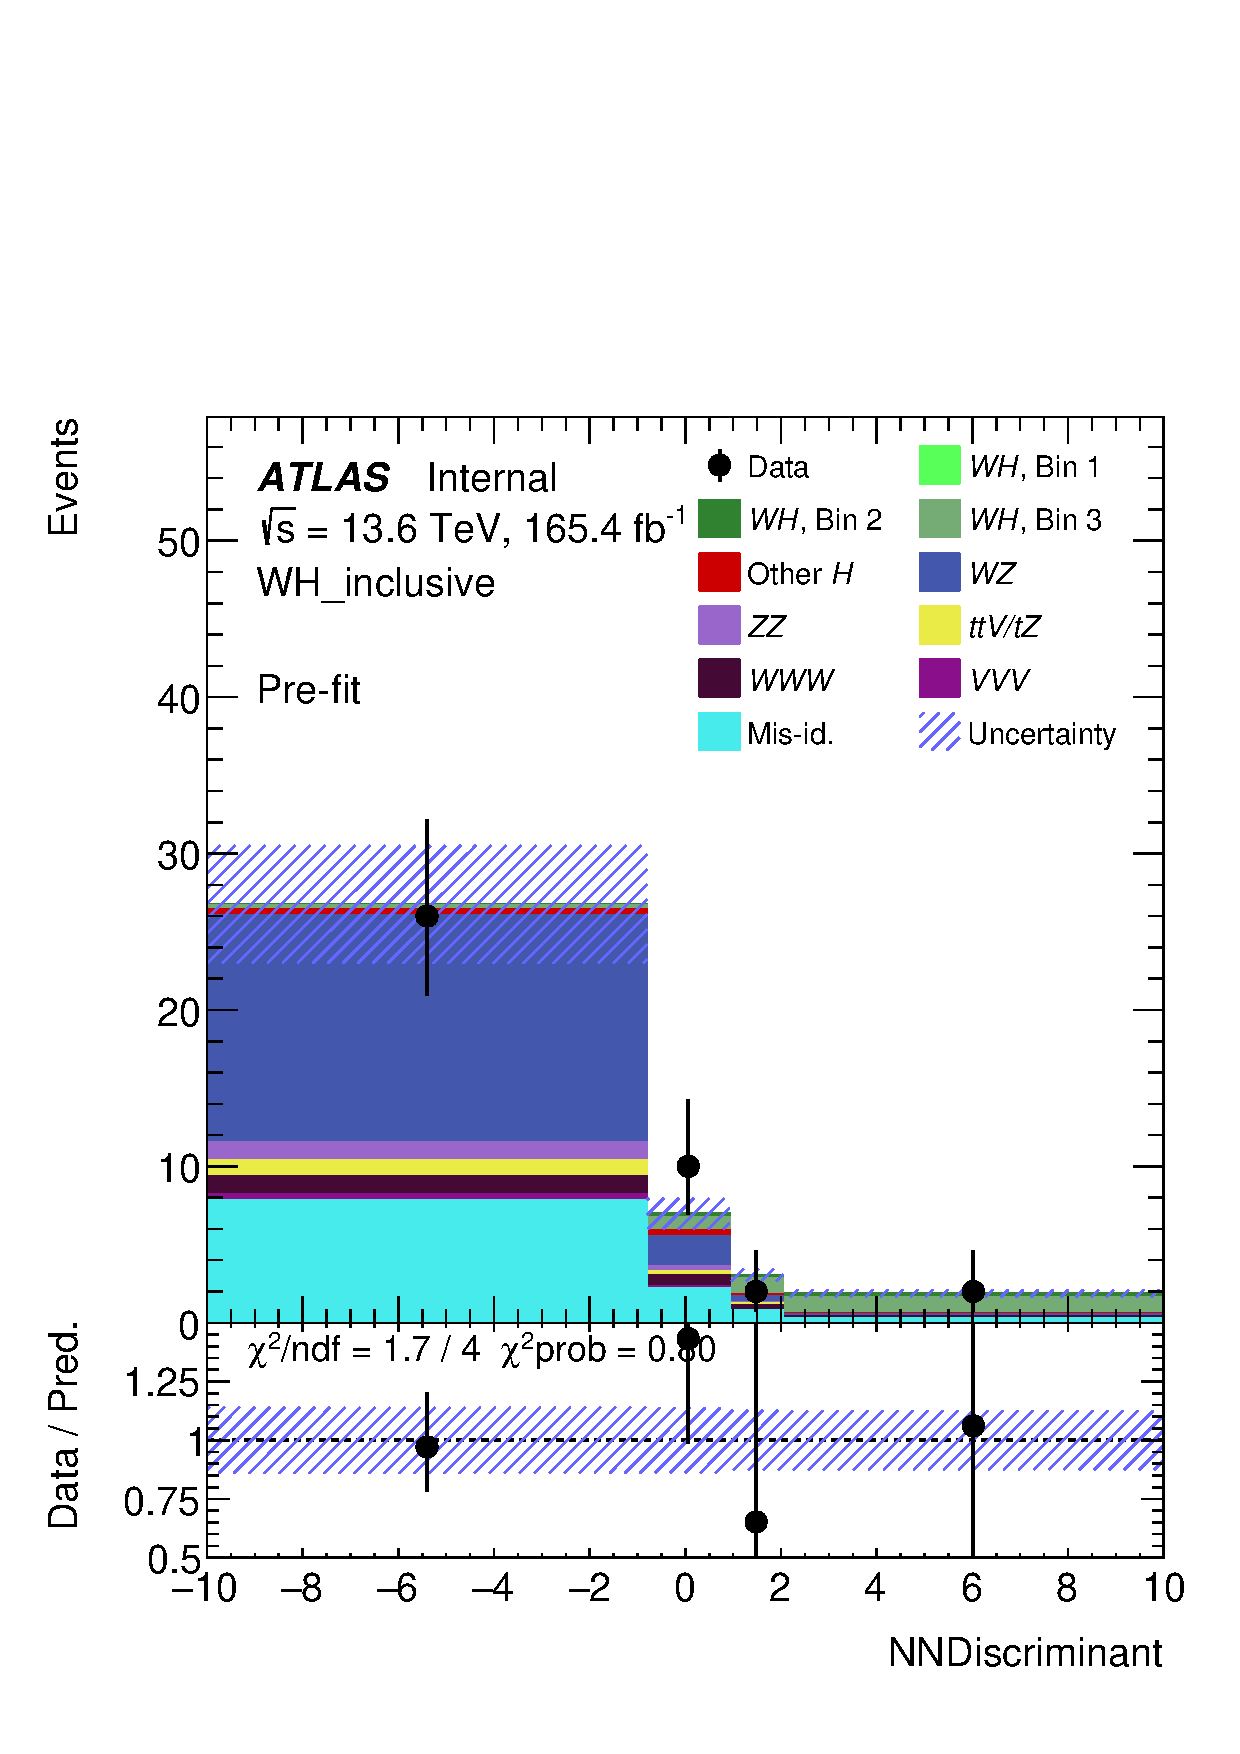
\includegraphics[width=0.4\textwidth]{figures/VH/VH_zdep_nn_discriminant_150toinf.pdf}\label{fig:vh_wh_zdep_www_discriminant_150toinf}
  }
  \caption{ANN discriminant for the \zdep{} SR split by the transverse momentum of the associated $W$ boson.}\label{fig:vh_wh_zdep_discriminant}
\end{figure}